% Figure 20 - MOM interaction class structure
% Independently reconstructed from IEEE Std 1516.1-2010 source physical p.263 / standard p.249.
% Diagram geometry uses the embedded source stencil's natural 960 x 720 coordinate system.
% Relationship IDs correspond to audit/figure20/relationships.csv.
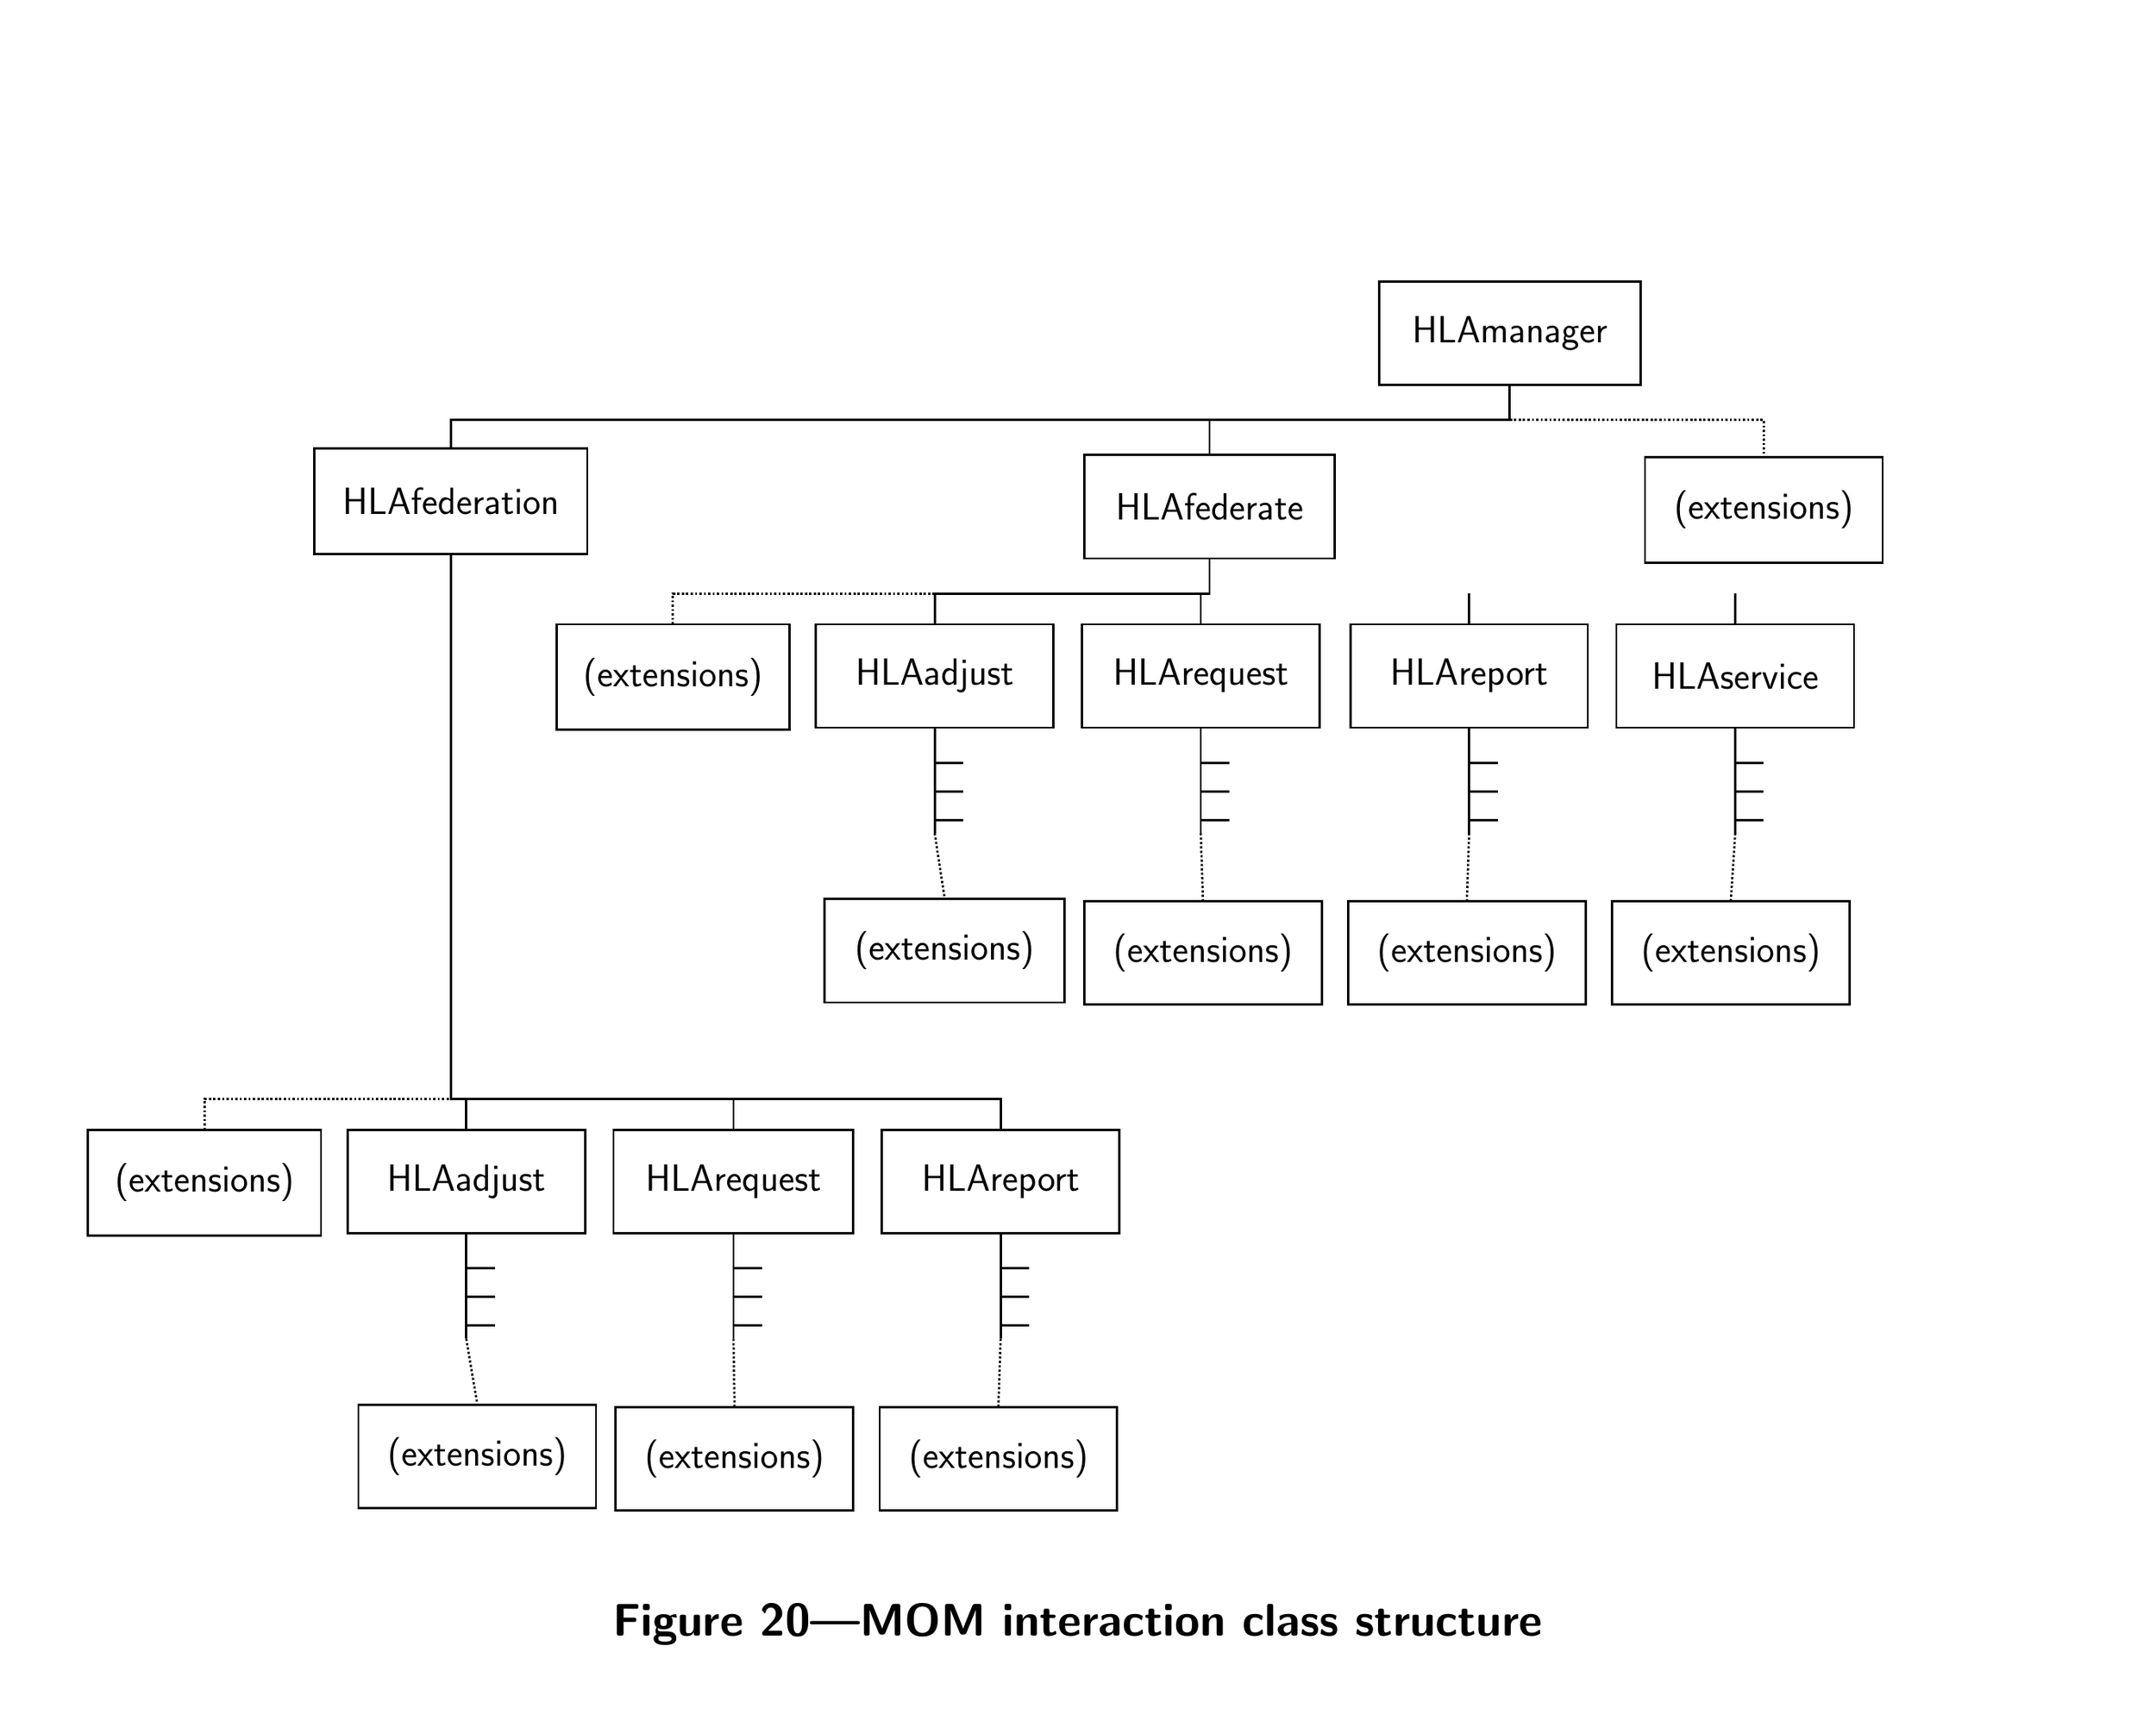
\begin{tikzpicture}[x=1pt,y=-1pt,line cap=butt,line join=miter]
    \path[use as bounding box] (0,0) rectangle (960,760);
    \tikzset{
        fbox/.style={draw,line width=1pt,inner sep=0pt,font=\sffamily\fontsize{17}{17}\selectfont,align=center},
        solid/.style={line width=1pt},
        dotted/.style={densely dotted,line width=1pt}
    }
    % Source-measured predefined and extension boxes.
    \node[fbox,minimum width=119pt,minimum height=47pt] (manager) at (676.5,141.5) {HLAmanager};
    \node[fbox,minimum width=124pt,minimum height=48pt] (federation) at (195,218) {HLAfederation};
    \node[fbox,minimum width=114pt,minimum height=47pt] (federate) at (540,220.5) {HLAfederate};
    \node[fbox,minimum width=108pt,minimum height=48pt] (mgrExt) at (792,222) {(extensions)};

    \node[fbox,minimum width=106pt,minimum height=48pt] (fedExt) at (296,298) {(extensions)};
    \node[fbox,minimum width=108pt,minimum height=47pt] (fAdj) at (415,297.5) {HLAadjust};
    \node[fbox,minimum width=108pt,minimum height=47pt] (fReq) at (536,297.5) {HLArequest};
    \node[fbox,minimum width=108pt,minimum height=47pt] (fRep) at (658,297.5) {HLAreport};
    \node[fbox,minimum width=108pt,minimum height=47pt] (fSvc) at (779,297.5) {HLAservice};

    \node[fbox,minimum width=109pt,minimum height=47pt] (fAdjExt) at (419.5,422.5) {(extensions)};
    \node[fbox,minimum width=108pt,minimum height=47pt] (fReqExt) at (537,423.5) {(extensions)};
    \node[fbox,minimum width=108pt,minimum height=47pt] (fRepExt) at (657,423.5) {(extensions)};
    \node[fbox,minimum width=108pt,minimum height=47pt] (fSvcExt) at (777,423.5) {(extensions)};

    \node[fbox,minimum width=106pt,minimum height=48pt] (gExt) at (83,528) {(extensions)};
    \node[fbox,minimum width=108pt,minimum height=47pt] (gAdj) at (202,527.5) {HLAadjust};
    \node[fbox,minimum width=109pt,minimum height=47pt] (gReq) at (323.5,527.5) {HLArequest};
    \node[fbox,minimum width=108pt,minimum height=47pt] (gRep) at (445,527.5) {HLAreport};
    \node[fbox,minimum width=108pt,minimum height=47pt] (gAdjExt) at (207,652.5) {(extensions)};
    \node[fbox,minimum width=108pt,minimum height=47pt] (gReqExt) at (324,653.5) {(extensions)};
    \node[fbox,minimum width=108pt,minimum height=47pt] (gRepExt) at (444,653.5) {(extensions)};

    % F20-R01..R03: manager-level predefined hierarchy and extension.
    \draw[solid] (676.5,165) -- (676.5,181) -- (195,181) -- (195,194); % F20-R01
    \draw[solid] (540,181) -- (540,197); % F20-R02
    \draw[dotted] (676.5,181) -- (792,181) -- (792,198); % F20-R03

    % F20-R04..R08: HLAfederate family.
    \draw[solid] (540,244) -- (540,260) -- (415,260) -- (415,274); % F20-R04
    \draw[solid] (536,260) -- (536,274); % F20-R05
    \draw[solid] (658,260) -- (658,274); % F20-R06
    \draw[solid] (779,260) -- (779,274); % F20-R07
    \draw[dotted] (415,260) -- (296,260) -- (296,274); % F20-R08

    % F20-R09..R12: omitted predefined subclasses then dotted extensions.
    \foreach \x/\ext in {415/fAdjExt,536/fReqExt,658/fRepExt,779/fSvcExt}{
        \draw[solid] (\x,321) -- (\x,369);
        \draw[solid] (\x,337) -- +(13,0);
        \draw[solid] (\x,350) -- +(13,0);
        \draw[solid] (\x,363) -- +(13,0);
        \draw[dotted] (\x,369) -- (\ext.north);
    }

    % F20-R13..R16: long HLAfederation family trunk and branch.
    \draw[solid] (195,242) -- (195,490) -- (202,490) -- (202,504); % F20-R13
    \draw[solid] (202,490) -- (323.5,490) -- (323.5,504); % F20-R14
    \draw[solid] (323.5,490) -- (445,490) -- (445,504); % F20-R15
    \draw[dotted] (202,490) -- (83,490) -- (83,504); % F20-R16

    % F20-R17..R19: lower omitted-subclass stems and extensions.
    \foreach \x/\ext in {202/gAdjExt,323.5/gReqExt,445/gRepExt}{
        \draw[solid] (\x,551) -- (\x,599);
        \draw[solid] (\x,567) -- +(13,0);
        \draw[solid] (\x,580) -- +(13,0);
        \draw[solid] (\x,593) -- +(13,0);
        \draw[dotted] (\x,599) -- (\ext.north);
    }

    \node[font=\sffamily\bfseries\fontsize{22}{24}\selectfont] at (480,729)
        {Figure 20---MOM interaction class structure};
\end{tikzpicture}
